\section{Réalisation}

\subsection{Requêtes analytiques}

Traitements : 
\begin{itemize}
    \item On cherche à savoir quel fromage est le plus vendu dans le sud est de la France.
    \item On veut savoir quel duo vin-charcuterie est le plus vendu en France, afin de pouvoir faire une remise dessus.
    \item On veut chercher les clients résidant en région parisienne qui ont déjà une remise actuellement active afin de ne pas leur en offrir une 2ème.
    \item On cherche à savoir quel est la région ou la clientèle est la plus importante, et celle qui est la moins importante, afin de faire des remises sur ces régions.
    \item On veut savoir quel plate-forme est la plus utilisée parmi nos clients.
    \item On cherche à savoir quel produit a été vendu le plus pour chaque région et pour chaque produit, afin de définir des box promotionnels.
    \item On cherche à savoir quel région a eu le plus de remise, afin de diminuer le nombre de ces dernières dans cette région.
    \item On cherche à savoir si notre clientèle est plutôt vieille ou jeune afin de faire profiter d'une certaines remises pour ces tranches d'âge.
    \item On cherche les produits les moins vendus par type, afin de potentiellement les supprimer de notre menu.
    \item Inversement, on cherches les produits les plus vendus par type, afin d'augmenter notre stock de ces produits.
\end{itemize}

    \begin{figure}[h]
        \centerline{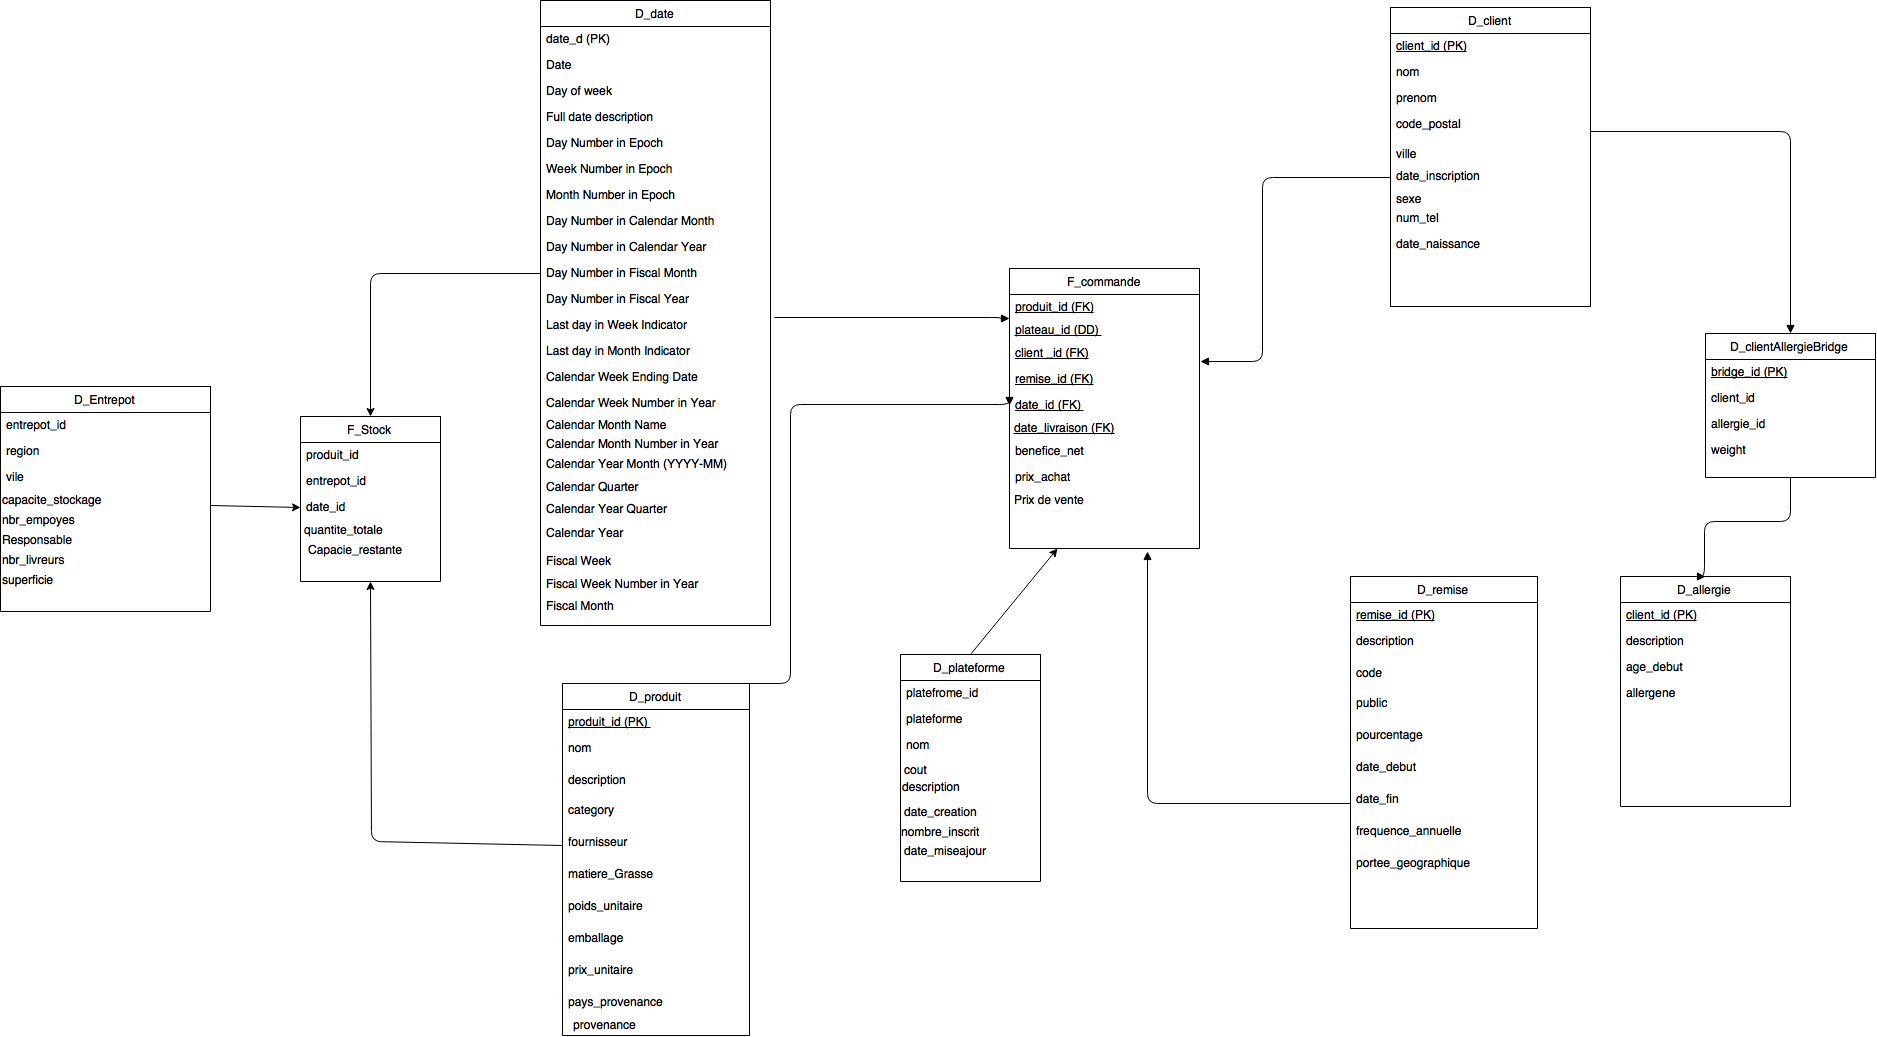
\includegraphics[scale=0.3]{Constelation.png}}
        \caption{Constellation de Datamarts}
        \label{fig:UML}
    \end{figure}
    
\subsection{Surrogate keys}
\paragraph{} Etant donné que l’utilisation des clés artificielles (Surrogate keys) est conseillée pour les tables dimensions. Nous avons choisi d’identifier les tuples insérés de façon incrémentale, en créant et utilisant des séquences pour l’insertion dans chaque table.

    \begin{figure}[h]
        \centerline{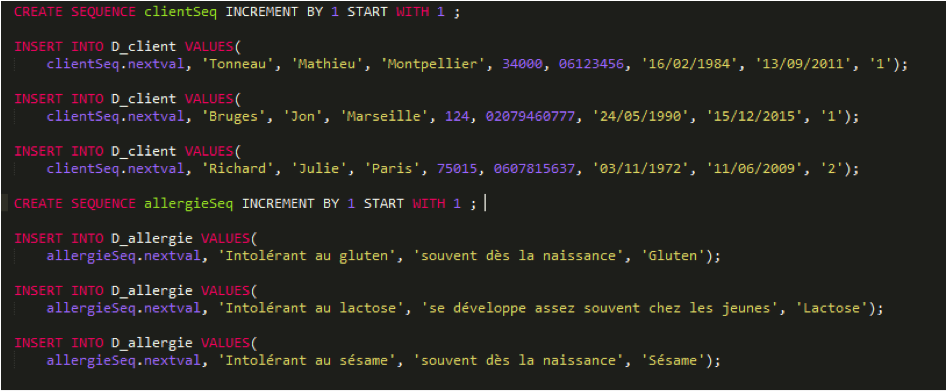
\includegraphics[scale=0.7]{Surrogate.png}}
        \caption{Surrogate keys}
        \label{fig:UML}
    \end{figure}

    
\subsection{Bridge tables (Multivaluated attributes)}
\paragraph{} Un attribut multi-valué est un attribut qui peut avoir plusieurs valeurs pour un seul tuple. Une occurrence de ce type d’attribut apparaît dans notre modèle, il s’agit de l’attribut allergie de la dimension "D\_client".
\paragraph{} Afin de gérer la multiplicité des valeurs possibles de l’attribut "allergie", nous avons dû faire intervenir une table pont (Bridge table) liant la dimension "D\_client" et la table allergie nouvellement créée.

    \begin{figure}[h]
        \centerline{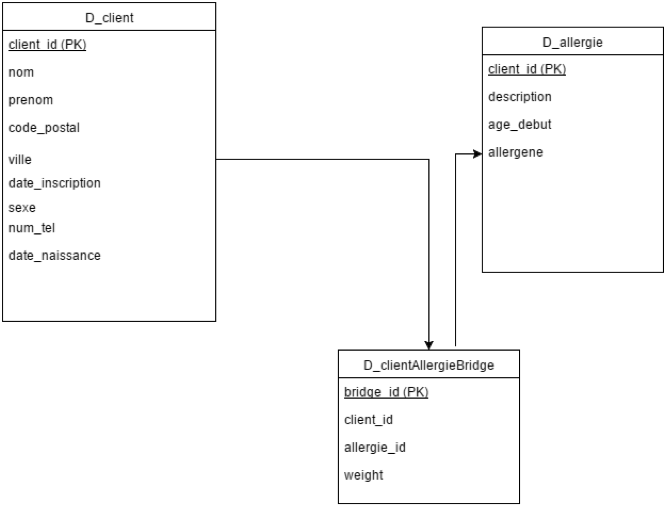
\includegraphics[scale=0.9]{schemaBridge.png}}
        \caption{Tables pont}
        \label{fig:UML}
    \end{figure}
    
    
\subsection{Vues virtuelles (Role-playing)}
\paragraph{} Étant donné que quelques dimensions sont partagées par les deux datamarts (en l’occurrence D\_produit et D\_date), les deux devront "jouer les rôles" de dimensions pour chacune des tables de faits des deux datamarts.

    \begin{figure}[h]
        \centerline{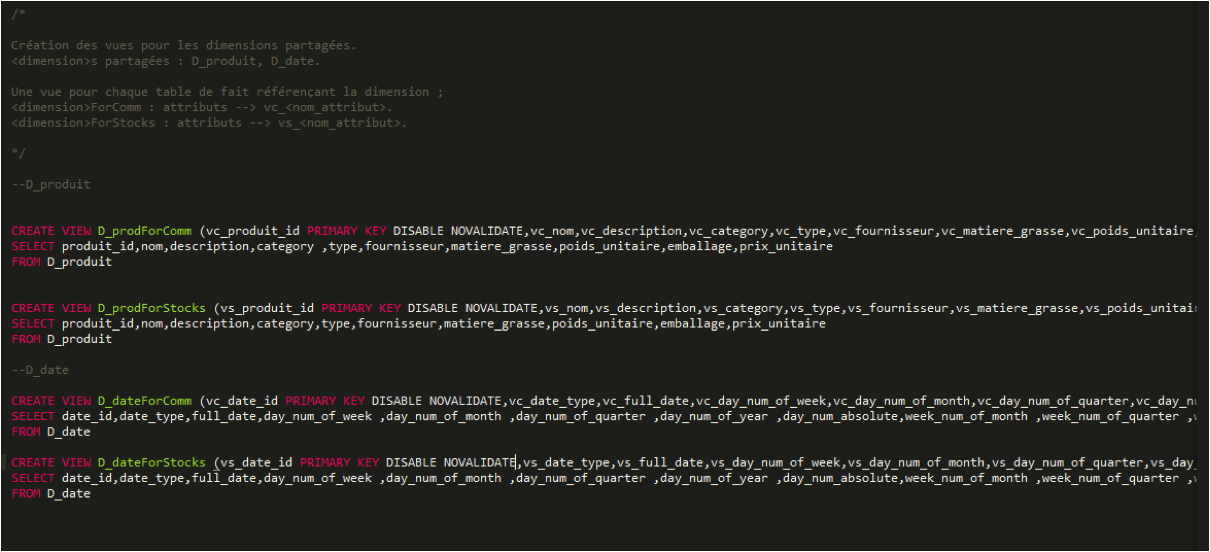
\includegraphics[scale=0.9]{screenTerm1.png}}
        \caption{Creation de vues}
        \label{fig:UML}
    \end{figure}
    
\newpage

\subsection{Problème d'insertion Oracle} 
\paragraph{} Après l’étape de création des tables de faits et des dimensions des deux datamarts, nous avons malheureusement rencontré un problème que nous n’avons pas pu contourner lors des insertions de tuples dans les tables. La capture d’écran suivante montre le message d’erreur affiché à chaque tentative d’insertion.


    \begin{figure}[h]
        \centerline{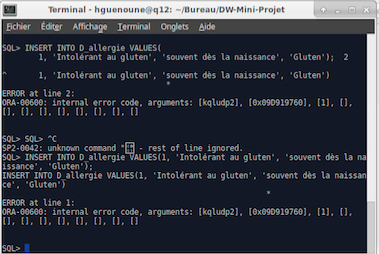
\includegraphics[scale=0.7]{error.png}}
        \caption{Erreur lors de l'insertion dans la base}
        \label{fig:UML}
    \end{figure}
